
\subsubsection{Location}
\label{sec:Location}
The \sbol{Location} class is extended by the \sbol{Range}, \sbol{Cut}, and \sbol{EntireSequence} classes.

\begin{figure}[ht]
\begin{center}
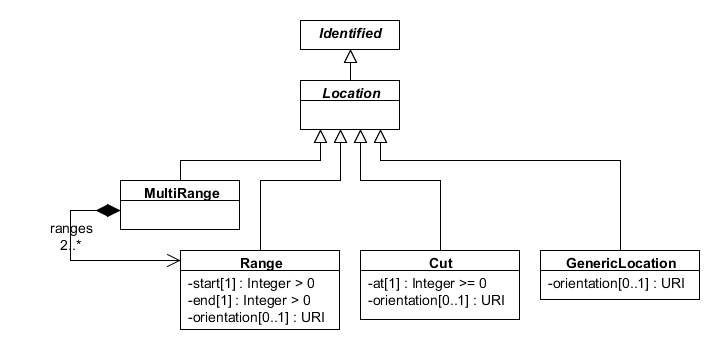
\includegraphics[scale=0.6]{uml/location}
\caption[]{Diagram of the \sbol{Location} class and its associated properties.}
\label{uml:location}
\end{center}
\end{figure} \todo{change diagram to reflect changes from SEP 41}

\subparagraph{The \sbolheading{orientation} property}
\label{sec:orientation}
The \sbol{orientation} property is OPTIONAL and has a data type of \sbol{URI}. All subclasses of \sbol{Location} share this property, which can be used to indicate how the region specified by the \sbol{SequenceFeature} and any associated double-stranded \sbol{Feature} is oriented on the \sbol{elements} of a \sbol{Sequence}  from their parent \sbol{Component}. \ref{tbl:orientation_types} provides a list of REQUIRED \sbol{orientation} \sbol{URI}s. If a \sbol{Location} object has an \sbol{orientation}, then it MUST come from \ref{tbl:orientation_types}.

\subparagraph{The \sbolheading{sequence} property}
\label{sec:sequence}
The \sbol{sequence} property is REQUIRED and MUST contain the \sbol{URI} of a \sbol{Sequence} object. All subclasses of \sbol{Location} share this property, which indicates which \sbol{Sequence} object referenced by the containing \sbol{Component} is referenced by the \sbol{Location}.

\begin{table}[ht]
  \begin{edtable}{tabular}{lp{3.75in}}
    \toprule
    \textbf{Orientation URI} & \textbf{Description} \\
    \midrule
    \url{http://sbols.org/v2\#inline} & The region specified by this \sbol{Location} is on the \sbol{elements} of a \sbol{Sequence}. \\
    \url{http://sbols.org/v2\#reverseComplement} & The region specified by this \sbol{Location} is on the reverse-complement translation of the \sbol{elements} of a \sbol{Sequence}. The exact nature of this translation depends on the \sbol{encoding} of the \sbol{Sequence}. \\
    \bottomrule
  \end{edtable}
  \caption{REQUIRED \sbol{URI}s for the \sbol{orientation} property}
  \label{tbl:orientation_types}
\end{table}


\paragraph{Range}
\label{sec:Range}
A \sbol{Range} object specifies a region via discrete, inclusive \sbol{start} and \sbol{end} positions that correspond to indices for characters in the \sbol{elements} \sbol{String} of a \sbol{Sequence}.

Note that the index of the first location is 1, as is typical practice in biology, rather than 0, as is typical practice in computer science.

\subparagraph{The \sbolheading{start} property}\label{sec:start}
The \sbol{start} property specifies the inclusive starting position of the \sbol{Range}. This property is REQUIRED and MUST contain an \sbol{Integer} value greater than zero.

\subparagraph{The \sbolheading{end} property}\label{sec:end}
The \sbol{end} property specifies the inclusive ending position of the \sbol{Range}. This property is REQUIRED and MUST contain an \sbol{Integer} value greater than zero. In addition, this \sbol{Integer} value MUST be greater than or equal to that of the \sbol{start} property.

\paragraph{Cut}
\label{sec:Cut}
The \sbol{Cut} class has been introduced to enable the specification of a region between two discrete positions.
This specification is accomplished using the \sbol{at} property, which specifies a discrete position that that corresponds to the index of a character in the \sbol{elements} \sbol{String} of a \sbol{Sequence} (except in the case when \sbol{at} is equal to zero---see below).

\subparagraph{The \sbolheading{at} property}
\label{sec:at}
The \sbol{at} property is REQUIRED and MUST contain an \sbol{Integer} value greater than or equal to zero. The region specified by the \sbol{Cut} is between the position specified by this property and the position that immediately follows it. When the \sbol{at} property is equal to zero, the specified region is immediately before the first discrete position or character in the \sbol{elements} \sbol{String} of a \sbol{Sequence}.


\paragraph{EntireSequence}
\label{sec:EntireSequence}
The \sbol{EntireSequence} class does not have any additional properties. Use of this class indicates that the linked Sequence describes the entirety of the \sbol{Component} or \sbol{Feature} parent of this Location object.

\subparagraph{The \sbolheading{order} property}
\label{sec:order}

